%
% $RCSfile$
%
% Copyright (c) 2005-2006. Christian Heller. All rights reserved.
%
% Permission is granted to copy, distribute and/or modify this document
% under the terms of the GNU Free Documentation License, Version 1.1 or
% any later version published by the Free Software Foundation; with no
% Invariant Sections, with no Front-Cover Texts and with no Back-Cover
% Texts. A copy of the license is included in the section entitled
% "GNU Free Documentation License".
%
% http://www.cybop.net
% - Cybernetics Oriented Programming -
%
% http://www.resmedicinae.org
% - Information in Medicine -
%
% Version: $Revision$ $Date$ $Author$
% Authors: Christian Heller <christian.heller@tuxtax.de>
%

\subsubsection{Data Garden}
\label{data_garden_heading}

Now, if a distinction of high-level knowledge from low-level system control
software is considered to be useful, the next question must be: \textit{How,
that is in which form, best to store knowledge in a system?}

One possible structure called \emph{Data Garden} \cite{holland} was proposed by
Wau Holland of the \emph{Chaos Computer Club} (CCC). Although being a
non-academic organisation, his ideas on knowledge modelling are interesting to
this work. He dreamt of whole \emph{Forests}, \emph{Parks} or -- as the name
says -- \emph{Gardens} of \emph{Knowledge Trees} and \emph{Data Bushes} (figure
\ref{garden_figure}).

\begin{figure}[ht]
    \begin{center}
        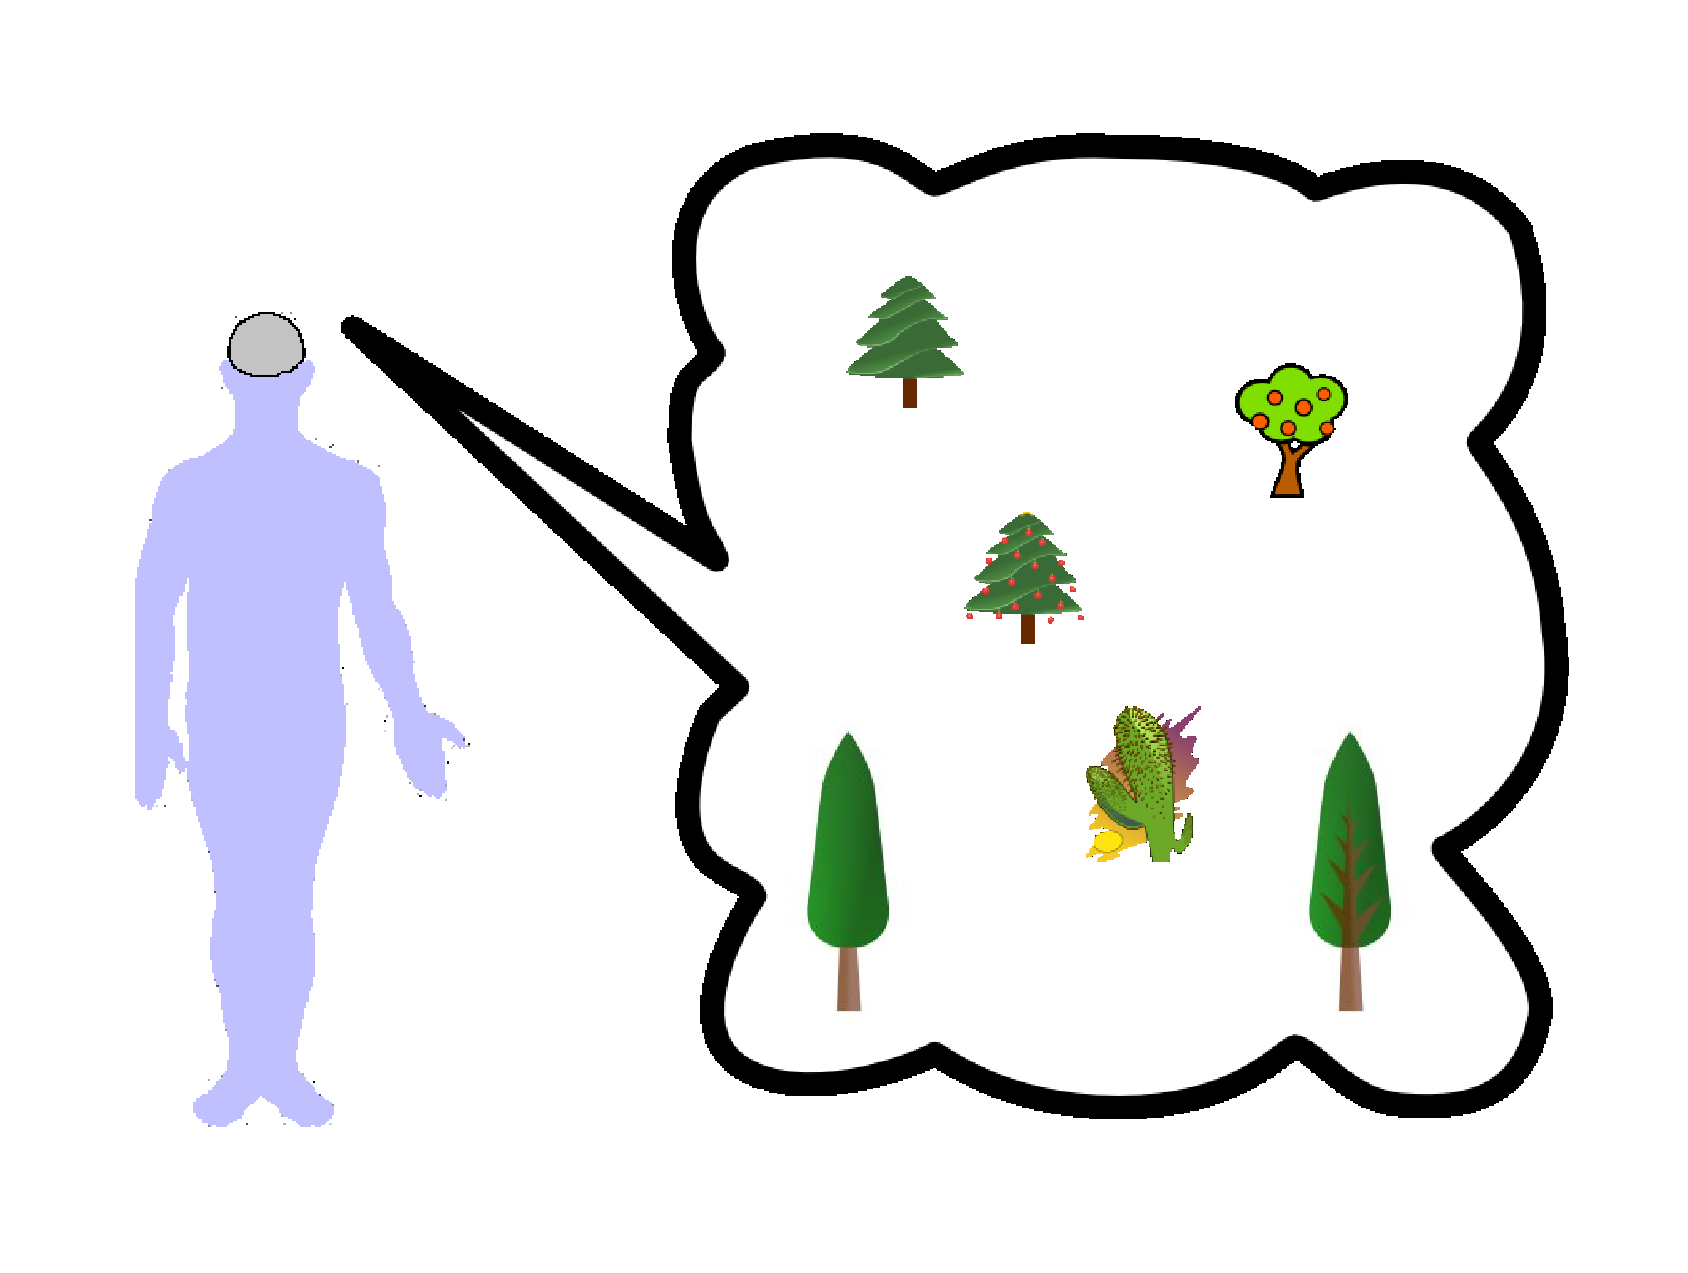
\includegraphics[scale=0.2]{vector/garden.eps}
        \caption{Data Garden}
        \label{garden_figure}
    \end{center}
\end{figure}

The interpreter (section \ref{cyboi_heading}) created in the work described in
this article stores all its knowledge in \emph{one single} tree, whose root
node it references. The single concepts (data bushes) are represented by
branches of that knowledge tree.
